
\section*{Control Mechanisms}
Given the possibility that swarming entities can operate autonomously, manually controlled, or both, there has been much research and reporting on their control systems which has driven the development of decentralized and centralized control architectures. These components play a significant role in the interaction between individual swarm agents, including their designated actions which can be based on information dictated, exchanged, and acquired. The operational efficiency of the distribution of tasks can be attributed to features such as hardware, software (intelligence algorithms, if any), capacity, and environment []. Abdelkader et al. (2021) presented a summary of the main applications related to aerial swarm systems and the associated research works detailing the main components of any swarm system, localization, and mission planning [18]. The group proposed an abstraction of an aerial swarm system architecture that can help developers to understand the main required modules. For distributed swarm systems with a centralized control architecture that includes a human-in-the-loop (HITL) it is suggested that a structure noted in Figure 4A, should be used for units with less capability of functionality. In this regime, various robots carry out their respective tasks locally while coordinating with one another via local communications and sensing.


 Small multi-UAV systems that lack the individual robot on-board capacity to complete swarm-level mission planning tasks may find utility for this architecture. On the contrary, for decentralized swarm systems, it was proposed that a more distributed model in which there is autonomy in place of the manual operator, allowing the entity’s memory and acquired information transmitted over networks to determine mission success. A detailed representation of this architecture is shown in Figure 4B. The latter model sets the platform for emergent behavior within the swarm, which enables the collection of agents to intelligently deduce optimal problem solutions in real-time. 

 
The knowledge of swarm control mechanisms is of critical importance in understanding overall swarm behavior, as it governs the method(s) agent for mission success. Typically, this would be categorized as centralized – i.e., where the command/control (C2) is in one location and commands and observations from the elements of the swarm are fused to provide a cohesive view for situational awareness, or decentralized where each element has some form of independent function and goal achievement which is coordinated by some form of message passing. The latter function is typically deemed as being computed ‘at the edge’. Communication to/from each element and to the command center (whether centralized or not) is critical. These tend to be encrypted, and while jamming is a possibility to counter a swarm, knowledge of which frequencies to jam is itself a (separate) problem. A third component of control is the potential role of one or more human-in-the-loop (HITL) [].

\begin{figure}[!h]
  \centering
  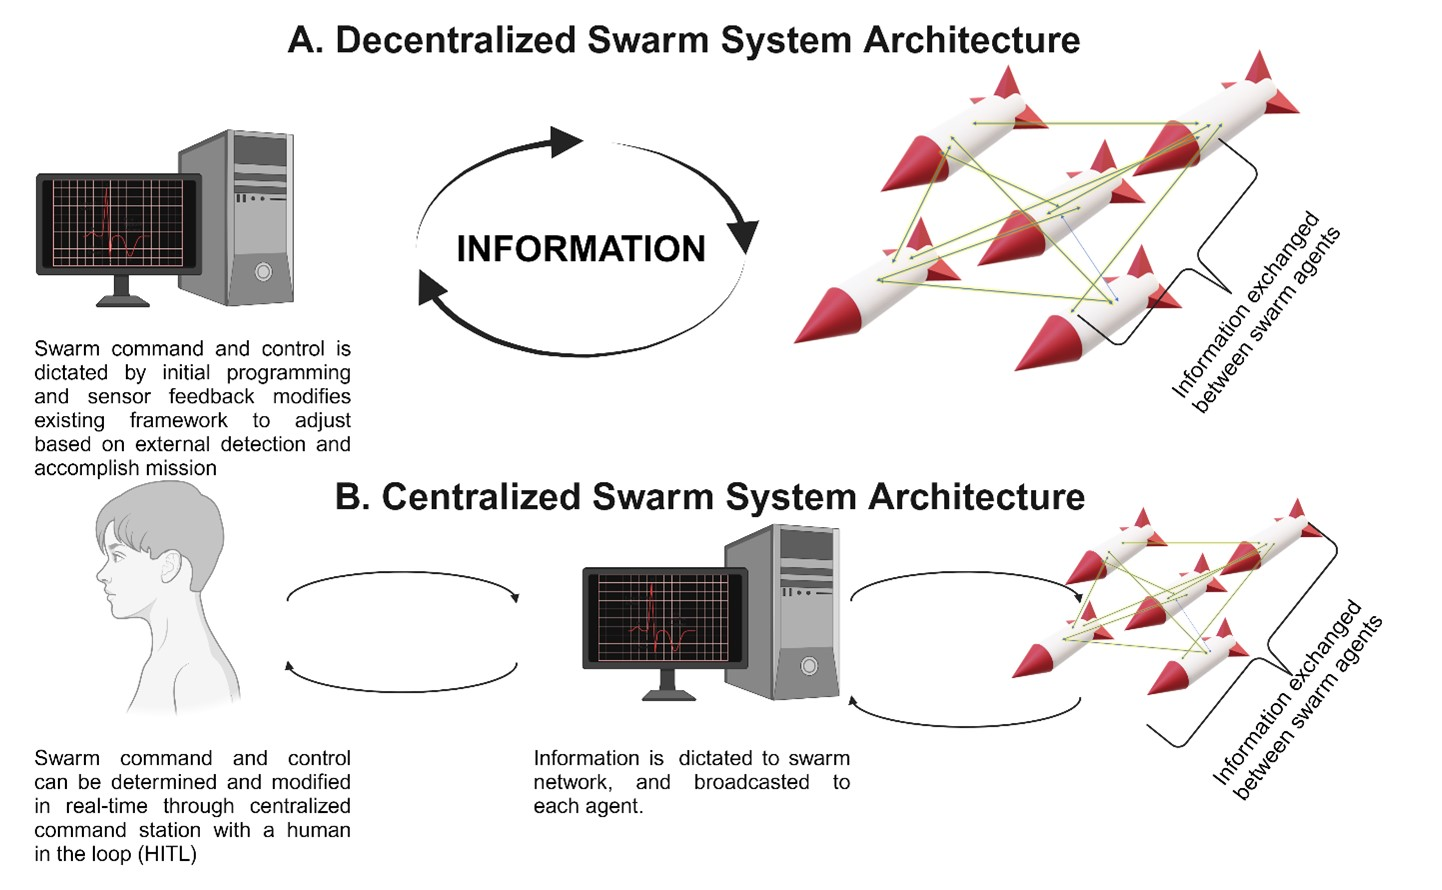
\includegraphics[width=0.7\textwidth]{control.jpg}
  \caption{Illustrations outlining some key differences between A) decentralized control architectures, and B) centralized control architectures in swarm systems. }
  \label{fig:platforms}
\end{figure}

Mixed - initiative control is a control paradigm where the machine (or in this case the ensemble) works with the human(s) for goal achievement. The role of the human(s) can be critical and potentially augmentative as an element of perception of the sensory feed, but also disruptive in how the individual can potentially preempt or even interfere in execution. A fourth issue relates to how goals are designated and tracked over time. This could be via simple visual interfaces and in homogeneous swarms relatively simple to use and observe at the C2 site. A typical diagram outlining some key fundamental differences between decentralized (autonomous) and centralized (HITL) control architectures are depicted in Figure 4. It is evident that information exchange is a major component in self-organized control systems, and the collection/receiving protocol for both system types are reversible [].


With heterogeneous elements in the swarm, assigning tasks can become more complex and is in of itself, a separate area of interest. Failure and recovery are a fifth element of task execution of swarms. The fundamental notion here is how to detect failures and to “reconfigure” the swarm in ways that as an ensemble, the swarm continues towards the goal(s) it/they was/were meant to achieve. This too is a separate area of study for single and multiple vehicles and non-trivial in its scope. With the notions above, the role of advanced automation using percepts of automated planning/scheduling and execution come into play, for control, for goal achievement as well (and critically so) in failure identification and recovery (FDIR – fault detection, identification, and recovery). Single agent autonomous operations typically are designed to deal with these issues, but the complexity rises when more than one robot/entity is in question. Methods such as T-REX, which is a multi-threaded controller with multiple control loops have achieved full-functional autonomous control of ground, aerial and underwater vehicles (AUVs) with compute on the “edge”, i.e., in-situ. Using a radio interface T-REX has also been used for HITL (mixed-initiative control) for operational AUVs. Other methods, again for single agent control, have been tried out in various stages of experimentation and settings. Development of operational control schema is a current challenge in swarm robotics.
